\documentclass[twocolumn]{article}
\usepackage{amsmath}
\usepackage{amssymb}
\usepackage{graphicx}

\begin{document}

\section*{Financial Mathematics}

\begin{itemize}
\item  The formula to calculate the simple interest is $I=\frac{P R T}{100}$, where 

$I=$ total simple interest earned or payable,

$P=$ principal amount (original or starting amount),

$R=$ rate of interest per annum (eg. if $4.5\%$ per annum, then $R=4.5$),

$T=$ number of years (eg. if $18$ months, then $T=1.5$).

\item The formula to calculate compound interest is $A=P\left(1+\frac{r}{100}\right)^n$, where 

$A=$ total amount after $n$ units of time,

$P=$ principal amount (original or starting amount),

$r=$ rate of interest (eg. if $2.4\%$, then $r=2.4$),

$n=$ number of units of time.

Example: $3$ years, $4.5 \%$ per annum:

$A = P\left(1+\frac{4.5}{100}\right)^3$

Example: Suppose the year is divided into $m$ equal sub-intervals. For quarterly compounding $m=4$. For monthly compounding, $m=12$. For semi-annual compounding, $m=2$. Then if $r$ denotes interest rate {\bf per annum} and $n$ denotes number of {\bf years},

$A=P\left(1+\frac{r/m}{100}\right)^{nm} = P\left(1+\frac{r}{100m}\right)^{nm}$

\item 

Profit $=$ Selling Price - Cost Price

\item If sold at below cost, then:

Loss $=$ Cost Price - Selling Price

\item 

$\%$ Profit or Loss $=\frac{\text { Profit or Loss }}{\text { Cost price }} \times 100 \%$

Cost price is regarded as $100 \%$

\item In absense of GST, {\bf marked price} refers to {\bf orginal selling price}

Discount $=$ Marked Price - Discounted Sales Price

\item  $\% \text { Discount }=\frac{\text { Discount }}{\text { Marked Price }} \times 100 \%$

$=\frac{\text { Marked Price - Discounted Sales Price }}{\text { Marked Price }} \times 100 \%$

Marked price is regarded as $100 \%$

\item In presence of GST, marked price {\bf includes} GST unless otherwise stated.

If GST is $9\%$, and the selling price before GST is regarded as $100\%$ then the marked price after GST is $109\%$.

Any discount imposed is on the marked price inclusive of GST.

\item Hire Purchase:

An initial down payment is made.

Simple interest is added to the {\bf remaining amount}, that is the amount left over after the down payment. Regard the {\bf principal amount} in the simple interest calculation as the {\bf amount left over after the down payment}.

Then the total balance to be paid {\bf inclusive of simple interest} is divided by the number of instalment periods to obtain the instalment amount per time period.

\item Income Tax example 1:

Use the tax rates given below to calculate the amount of tax Matthew and Tom have to pay.

(a) Matthew's annual chargeable income was $\$ 28500$. Tom's annual chargeable income was $\$ 37400$.

(b) Irene's income tax for last year was $\$ 499.60$. How much was her annual chargeable income last year?

\begin{tabular}{|l|c|c|}
	\hline Chargeable income (\$) & Rate (\%) & Tax Payable (\$) \\
	\hline On the first 20000 & 0 & 0 \\
	On the next 10000 & 2 & 200 \\
	\hline On the first 30000 & - & 200 \\
	On the next 10000 & 3.5 & 350 \\
	\hline
\end{tabular}

(a) 

Matthew:

Tax on the first $\$ 20000=\$ 0$

Tax on the next $\$ 8500=\frac{2}{100} \times \$ 8500=\$ 170$

Total tax $=\$ 0+\$ 170=\$ 170$

$\therefore \quad$ Matthew has to pay $\$ 170$ of tax.

Tom:

Tax on the first $\$ 30000=\$ 200$

Tax on the next $\$ 7400=\frac{3.5}{100} \times \$ 7400=\$ 259$

Total tax $=\$ 200+\$ 259=\$ 459$

$\therefore$ Tom has to pay $\$ 459$ of tax.

(b)

Irene:

$
\begin{aligned}
	& \text { Tax on the first } \$ 30000=\$ 200 \\
	& \begin{aligned}
		\text { Tax on the remainder } & =\$ 499.60-\$ 200 \\
		& =\$ 299.60
	\end{aligned}
\end{aligned}
$

Let $\$ x$ be the remainder.

$
\begin{aligned}
	\frac{3.5}{100} \times \$ x & =\$ 299.60 \\
	\$ x & =\frac{100}{3.5} \times \$ 299.60 \\
	& =\$ 8560
\end{aligned}
$

Annual chargeable income last year

$
\begin{aligned}
	& =\$ 30000+\$ 8560 \\
	& =\$ 38560
\end{aligned}
$

\item Income Tax example 2:

The table below shows the rates of income tax for 2018.

(a) Theresa's chargeable income for the year ended 2018 was $\$ 108000$. Calculate the amount of income tax she has to pay for 2018 .

(b) Theresa received a pay drop in 2019. The tax rate in 2019 is the same as 2018. Calculate her chargeable income in 2019 if her income tax payable in 2019 is $\$ 480$.

\begin{tabular}{|c|c|c|}
	\hline Chargeable Income & Rate $(\%)$ & Gross Tax Payable (\$) \\
	\hline First $\$ 20 000$ & 0 & 0 \\
	\hline Next $\$ 10000$ & 2 & 200 \\
	\hline First $\$ 30000$ & - & 200 \\
	\hline Next $\$ 10000$ & 3.50 & 350 \\
	\hline First $\$ 40000$ & - & 550 \\
	\hline Next $\$ 40000$ & 7 & 2800 \\
	\hline First $\$ 80000$ & - & 3350 \\
	\hline Next $\$ 40000$ & 11.5 & 4600 \\
	\hline
\end{tabular}

(a) 

$\$ 108000-\$ 80000=\$ 28000$

Tax on first $\$ 80000=\$ 3350$

Tax on next $\$ 28000=\frac{11.5}{100} \times \$ 28000=\$ 3220$

Total tax $=\$ 3350+\$ 3220 =\$ 6570$

(b) 

If income tax payable in 2019 is $\$ 480$, then she earns at least $\$ 30000$ but below $\$ 40000$ 

Tax on the remainder above $\$ 30000$

$
\begin{aligned}
	& =\$ 480-\$ 200 \\
	& =\$ 280
\end{aligned}
$

Let $\$ x$ be the remainder.

$
\begin{aligned}
	\frac{3.50}{100} \times \$ x & =\$ 280 \\
	\$ x & =\frac{100}{3.50} \times \$ 280 \\
	& =\$ 8000
\end{aligned}
$

Total chargeable income

$
\begin{aligned}
	& =\$ 30000+\$ 8000 \\
	& =\$ 38000
\end{aligned}
$

\end{itemize}

\newpage 

\section*{Vectors}

\begin{itemize}
	
\item  The vector below can be denoted by $\overrightarrow{A B}$.

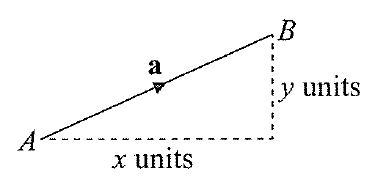
\includegraphics[width=0.3\textwidth]{201.png}

\item The magnitude/length of the vector is denoted by $|\overrightarrow{A B}|$ or $\left|\binom{x}{y}\right|$.

If $\mathbf{a}=\binom{x}{y}$, then its magnitude is given by:
$|\mathbf{a}|=\sqrt{x^2+y^2}$ (using Pythagoras' Theorem)

\item Position vectors:

A directed line segment $\overrightarrow{O P}$ indicates the position of a point $P$ taken with reference to the origin $O$. 

Vectors with the origin as their initial point are known as position vectors.

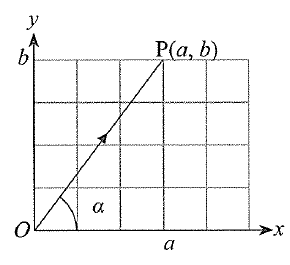
\includegraphics[width=0.3\textwidth]{202.png}

If the point $P$ has coordinates $(a, b)$, then the position vector of $P$ is $\overrightarrow{O P}=\binom{a}{b}$.

The magnitude or length of $O P$ is given by $|\overrightarrow{O P}|=\sqrt{a^2+b^2}$.

\item In the diagram below,

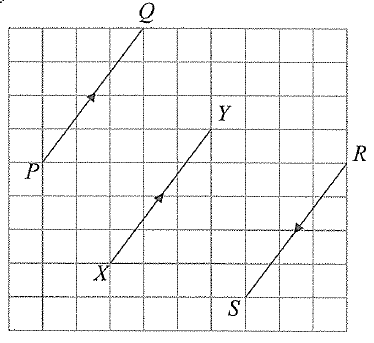
\includegraphics[width=0.3\textwidth]{203.png}

$
\overrightarrow{P Q}=\overrightarrow{X Y}
$

$\overrightarrow{R S}$ is the negative vector of $\overrightarrow{P Q}$.

$
\overrightarrow{P Q}=-\overrightarrow{R S}
$

Note that $|\overrightarrow{P Q}|=|\overrightarrow{R S}|$.

Zero or null vectors are vectors whose magnitude is zero. For example: $\overrightarrow{P Q}+\overrightarrow{R S}=\mathbf{0}$.

\item Sum of Two Vectors

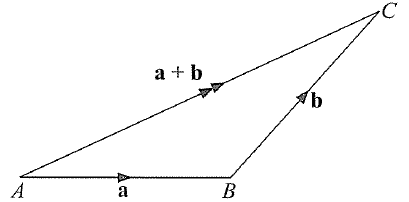
\includegraphics[width=0.3\textwidth]{204.png}

$\overrightarrow{A B}+\overrightarrow{B C}=\overrightarrow{A C}$

\item Difference of Two Vectors

$
\begin{aligned}
	\overrightarrow{A B} & =\overrightarrow{A O}+\overrightarrow{O B} \text { (using vector addition) } \\
	& = - \overrightarrow{O A}+\overrightarrow{O B} \text { (using negative vector } \overrightarrow{A O}=-\overrightarrow{O A} \text { ) } \\
	& =\overrightarrow{O B}-\overrightarrow{O A}
\end{aligned}
$

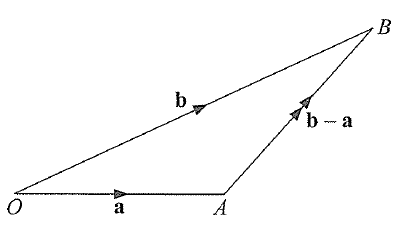
\includegraphics[width=0.3\textwidth]{205.png}

\item Translation:

If an object point $P(a, b)$, which can be expressed as $\overrightarrow{O P}=\binom{a}{b}$, undergoes a translation $T=\binom{h}{k}$, then the image point of $P$, i.e. $Q$ can be found by:

$
\begin{aligned}
	\overrightarrow{O Q} & =\overrightarrow{O P}+\binom{h}{k} \\
	& =\binom{a}{b}+\binom{h}{k} \\
	& =\binom{a+h}{b+k}
\end{aligned}
$

\item  Vector $\mathbf{a}$ is parallel to vector $\mathbf{b} \Leftrightarrow \mathbf{a}=k \mathbf{b}$, where $k$ is a scalar.

If $\mathbf{a}=k \mathbf{b}$, where $k$ is a scalar, then

(i) $|\mathbf{a}|=|k \| \mathbf{b}|$

(ii) If $k$ is positive, $\mathbf{a}$ and $\mathbf{b}$ are in the same direction. If $k$ is negative, $\mathbf{a}$ and $\mathbf{b}$ are in opposite directions.

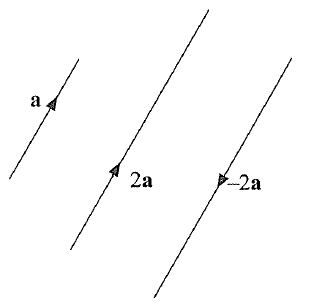
\includegraphics[width=0.3\textwidth]{206.png}

\item Suppose $\mathbf{a}$ and $\mathbf{b}$ are non-parallel vectors, and $h, k, m$ and $n$ are scalars.

(i) If $h \mathbf{a}=k \mathbf{b}$, then $h=0$ and $k=0$.

(ii) If $n \mathbf{a}+m \mathbf{b}=h \mathbf{a}+k \mathbf{b}$, then $n=h$ and $m=k$.

\item Points $A, B$ and $C$ are collinear, i.e. they lie on a straight line $\Leftrightarrow \ \overrightarrow{A B}=k \overrightarrow{B C}$

$\Leftrightarrow \ \overrightarrow{A B}=h \overrightarrow{A C}$ 

$\Leftrightarrow \ \overrightarrow{B C}=m \overrightarrow{A C}$


\end{itemize}




\end{document}


%  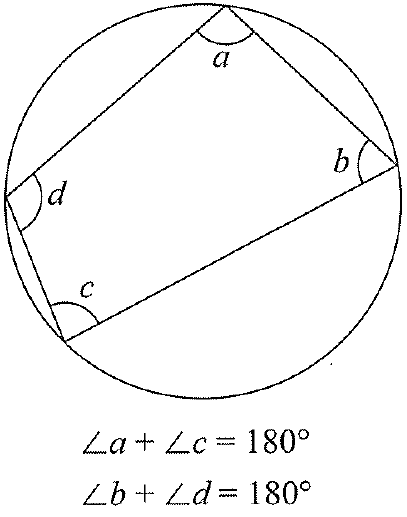
\includegraphics[width=0.25\textwidth]{152.png}


